\documentclass[tikz, border=5pt]{standalone}
\usepackage{amsmath} % For \text and math symbols
\usetikzlibrary{arrows.meta, positioning, fit, backgrounds, calc, matrix}

\begin{document}
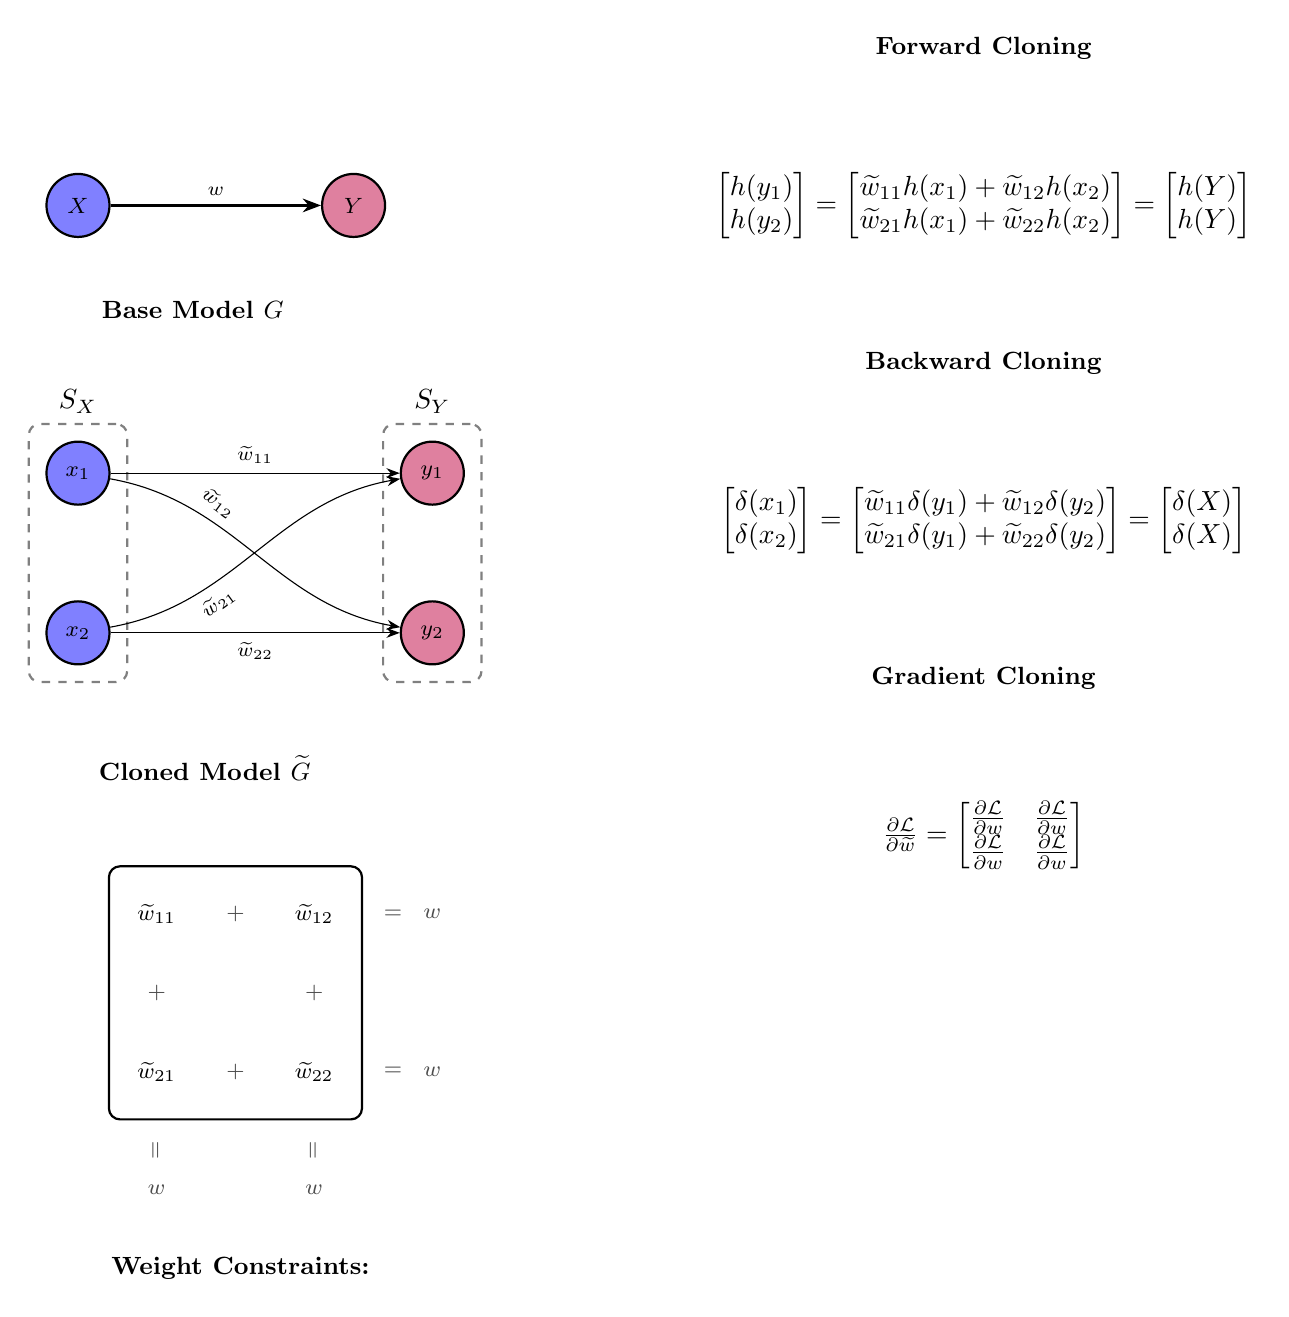
\begin{tikzpicture}[
    node_style/.style={circle, draw, thick, minimum size=0.8cm, font=\footnotesize},
    snode_x/.style={node_style, fill=blue!50},
    snode_y/.style={node_style, fill=purple!50}, % Using purple for the output layer
    partition_style/.style={draw, gray, dashed, thick, rounded corners, inner sep=6pt},
    edge_label_style/.style={midway, font=\scriptsize, black, sloped},
    grad_label_style/.style={midway, font=\scriptsize, blue!60!black, sloped},
    text_anno_style/.style={font=\footnotesize, align=left},
    row_title_style/.style={font=\bfseries, anchor=west},
    matrix_element/.style={minimum size=1.2cm, inner sep=0.3cm, font=\footnotesize},
    matrix_sum/.style={font=\footnotesize,opacity=0.7}
]

% LEFT COLUMN - GRAPHS AND WEIGHT CONSTRAINTS

% Base Graph
\begin{scope}[xshift=0cm, yshift=8cm]
    \node[snode_x] (b1x) at (0,0) {$X$};
    \node[snode_y] (b1y) at (3.5,0) {$Y$}; % Increased x-distance from X
    \node[font=\small\bfseries, below=0.3cm of b1x.south west, xshift=1.75cm, yshift=-0.5cm] {Base Model $G$};
    \draw[-Stealth, thick] (b1x) to node[edge_label_style, above] {$w$} (b1y);
\end{scope}

% Cloned Graph
\begin{scope}[xshift=0cm, yshift=4cm] % Changed yshift for vertical alignment
    \node[snode_x] (c1x1) at (0,0.6) {$x_1$}; % Slightly more y-separation
    \node[snode_x, below=1.2cm of c1x1] (c1x2) {$x_2$}; % Slightly more y-separation
    \node[snode_y] (c1y1) at (4.5,0.6) {$y_1$}; % Increased x-distance from S_X
    \node[snode_y, below=1.2cm of c1y1] (c1y2) {$y_2$};
    
    \begin{pgfonlayer}{background}
        \node[partition_style, fit=(c1x1) (c1x2), label=north:$S_X$] (p1sx) {};
        \node[partition_style, fit=(c1y1) (c1y2), label=north:$S_Y$] (p1sy) {};
    \end{pgfonlayer}
    \node[font=\small\bfseries, below=0.3cm of p1sx.south west, xshift=2.25cm, yshift=-0.5cm] {Cloned Model $\widetilde{G}$};

    % Edges S_X -> S_Y with more expressive curves
    \draw[-Stealth] (c1x1) to[out=0, in=180, looseness=0.8] node[edge_label_style, above] {$\widetilde{w}_{11}$} (c1y1);
    \draw[-Stealth] (c1x1) to[out=-10, in=170, ] node[edge_label_style, above left, pos=0.4] {$\widetilde{w}_{12}$} (c1y2);
    \draw[-Stealth] (c1x2) to[out=10, in=-170,] node[edge_label_style, below left, pos=0.4] {$\widetilde{w}_{21}$} (c1y1);
    \draw[-Stealth] (c1x2) to[out=0, in=180, looseness=0.8] node[edge_label_style, below] {$\widetilde{w}_{22}$} (c1y2);
\end{scope}

% Weight Matrix
\begin{scope}[xshift=0cm, yshift=-1cm] % Changed xshift and yshift for vertical alignment
    % Explanation title
    \node[font=\small\bfseries, anchor=west,xshift=0.3cm,yshift=-6cm] (title) at (0,1.5) {Weight Constraints:};
    
    % Create the matrix elements without individual boxes
    \node[matrix_element] (m11) at (1,0) {$\widetilde{w}_{11}$};
    \node[matrix_element] (m12) at (3,0) {$\widetilde{w}_{12}$};
    \node[matrix_element] (m21) at (1,-2) {$\widetilde{w}_{21}$};
    \node[matrix_element] (m22) at (3,-2) {$\widetilde{w}_{22}$};
    
    % Single rounded box around the matrix
    \node[draw, rounded corners, thick, fit=(m11) (m12) (m21) (m22), inner sep=0.0cm] (matrix_box) {};
    
    % Horizontal plus signs with equal distance
    \node[matrix_sum] (h_plus1) at (2,0) {$+$};
    \node[matrix_sum] (h_plus2) at (2,-2) {$+$};
    
    % Vertical plus signs with equal distance
    \node[matrix_sum] (v_plus1) at (1,-1) {$+$};
    \node[matrix_sum] (v_plus2) at (3,-1) {$+$};
    
    % Row sums - using fixed offset for symmetry
    \node[matrix_sum] (eq1) at (4,0) {$=$};
    \node[matrix_sum] (w1) at (4.5,0) {$w$};
    \node[matrix_sum] (eq2) at (4,-2) {$=$};
    \node[matrix_sum] (w2) at (4.5,-2) {$w$};
    
    % Column sums with rotated equal signs
    \node[matrix_sum, rotate=90] (veq1) at (1,-3) {$=$};
    \node[matrix_sum] (vw1) at (1,-3.5) {$w$};
    \node[matrix_sum, rotate=90] (veq2) at (3,-3) {$=$};
    \node[matrix_sum] (vw2) at (3,-3.5) {$w$};
\end{scope}

% RIGHT COLUMN - CLONING EQUATIONS

% Forward Cloning 
\begin{scope}[xshift=9cm, yshift=8cm] % Aligned with the Base Graph
    % Title for Forward Cloning
    \node[font=\small\bfseries, anchor=center] (fwd_title) at (2.5,2) {Forward Cloning};
    
    % Create a more compact equation for forward cloning
    \node (fwd_eq) at (2.5,0) {$
    \begin{bmatrix} h(y_1) \\ h(y_2) \end{bmatrix} = 
        \begin{bmatrix} \widetilde{w}_{11} h(x_1) + \widetilde{w}_{12} h(x_2) \\ 
        \widetilde{w}_{21} h(x_1) + \widetilde{w}_{22}  h(x_2)
        \end{bmatrix}  =
        \begin{bmatrix} h(Y) \\ h(Y) \end{bmatrix}$};
\end{scope}

% Backward Cloning
\begin{scope}[xshift=9cm, yshift=4cm] % Aligned with the Cloned Graph
    % Title for Backward Cloning
    \node[font=\small\bfseries, anchor=center] (bwd_title) at (2.5,2) {Backward Cloning};
    
    % Create a more compact equation for backward cloning
    \node (bwd_eq) at (2.5,0) {$\begin{bmatrix} \delta(x_1) \\ \delta(x_2) \end{bmatrix} = 
        \begin{bmatrix} \widetilde{w}_{11} \delta(y_1) + \widetilde{w}_{12}\delta(y_2) \\ \widetilde{w}_{21}\delta(y_1) +\widetilde{w}_{22}\delta(y_2) \end{bmatrix}   
        = 
        \begin{bmatrix} \delta(X) \\ \delta(X) \end{bmatrix}$};
\end{scope}

% Gradient Cloning
\begin{scope}[xshift=9cm, yshift=0cm] % Aligned with the Weight Constraints
    % Title for Gradient Cloning
    \node[font=\small\bfseries, anchor=center] (grad_title) at (2.5,2) {Gradient Cloning};
    
    % Gradient equation
    \node[anchor=center] (grad_eq) at (2.5,0) {
        $\frac{\partial \mathcal{L}}{\partial \widetilde{w}} =
        \begin{bmatrix}
        \frac{\partial \mathcal{L}}{\partial w} & \frac{\partial \mathcal{L}}{\partial w} \\
        \frac{\partial \mathcal{L}}{\partial w} & \frac{\partial \mathcal{L}}{\partial w}
        \end{bmatrix}$
    };
\end{scope}

\end{tikzpicture}
\end{document}